\chapter{Technologien}
\label{chap:technologies}

%%%%%%%%%%%%%%%%%%%%%%%%%%%%%%%%%%%%%%%%%%%%%%%%%%%%%%%%%%%%
\section{Bluetooth 4.0}
\label{sec:technologies:bluetooth4}
%%%%%%%%%%%%%%%%%%%%%%%%%%%%%%%%%%%%%%%%%%%%%%%%%%%%%%%%%%%%

Die Bluetooth-Version 4.0, oder auch Bluetooth Smart genannt, wurde 2009 final spezifiziert und wird seit Ende 2010 in Endgeräten eingesetzt.
Dieser Standard beinhaltet neben dem klassischen Bluetooth, eine neue Version, mit dem Namen Bluetooth Low Energy, welche, wie der Name schon andeutet, einen sehr viel geringeren Stromverbrauch vorweißt. Dabei ist der Stromverbrauch zwischen zwei und 100 mal geringer als beim klassischen Bluetooth.


%%%%%%%%%%%%%%%%%%%%%%%%%%%%%%%%%%%%%%%%%%%%%%%%%%%%%%%%%%%%
\section{Bluetooth Low Energy}
\label{sec:technologies:bluetoothLE}
%%%%%%%%%%%%%%%%%%%%%%%%%%%%%%%%%%%%%%%%%%%%%%%%%%%%%%%%%%%%

Bluetooth Low Energy wurde Anfangs von Nokia unter dem Namen ''Wibree'' entwickelt. Die Zielsetzung dabei war es eine Technologie zu entwickeln, mit der sich Computer und Mobilgeräte schnell und einfach mit Peripherie-Geräten verbinden lassen. Das Hauptaugenmerk galt dabei dem geringen Stromverbrauch, kompakter Bauweise und den Kosten für die benötigte Hardware.
Im Jahr 2007 wurden diese Spezifikationen dann in den, sich in der Entwicklung befindenden, Bluetooth-Standard 4.0 aufgenommen und daraufhin in Bluetooth Low Energy, oder kurz BLE umbenannt.

Bluetooth Low Energy arbeitet wie das klassische Bluetooth im 2,4 GHz Band, bringt aber in der Funktionsweise einige Unterschiede mit sich.

So wurde, im Vergleich zum klassischem Bluetooth, die Datenrate von bis zu 3 Mbit/s auf maximal 1 Mbit/s reduziert. Dies führt dazu, dass BLE zum Beispiel nicht für Headsets genutzt werden kann, da die zur Verffügung stehende Übertragungsrate nicht für die Audioübertragung ausreicht.

Die Vorteile die BLE mit sich bringt, liegen vor allem in der niedrigen Latenz, welche von 100ms auf bis zu unter 3ms reduziert wurde, und, wie bereits erwähnt, der Energieverbrauch drastisch gesenkt wurde.



Bluetooth Low Energy bietet darüber hinaus eine Vielzahl sogennanter GATT-Profile (Generic Attribute Profile). Die bereitgestellten GATT-Profile sind Richtlinen für die Bluetooth-Funktionialität, sprich, welche Daten übertragen werden und in welcher Form. Dies erlaubt eine einfache und schnell Interoperabilität zwischen verschiedenen Geräten. Ein Beispiel für ein GATT-Profil wäre zum Beispiel das ''Heart Rate Profile'', welches besipielsweise die Verbindung und Kommunikation eines Pulsmessgurtes mit einem Endgerät beschreibt. So wird sichergestellt, dass dieser Gurt mit jedem Endgerät auf die selbe Weise funktioniert.




%%%%%%%%%%%%%%%%%%%%%%%%%%%%%%%%%%%%%%%%%%%%%%%%%%%%%%%%%%%%
\subsection{iBeacons}
\label{sec:technologies:bluetoothLE:ibeacons}
%%%%%%%%%%%%%%%%%%%%%%%%%%%%%%%%%%%%%%%%%%%%%%%%%%%%%%%%%%%%
Die iBeacons-Technologie wurde am 10.Juni 2014 von Apple auf der Worldwide Developers Conference vorgestellt. 
Diese basiert auf Bluetooth Low Energy und arbeitet mit einem von Apple entwickelten GATT-Profil.

Beacon bedeutet übersetzt ''Leuchtfeuer'' und die Funktionsweise der Beacons ist dem sehr ähnlich.
Einmal in Betrieb genommen, sendet das Beacon kontinuierlich ein Signal, in welchem sich Daten zur Identifizierung des Beacons befinden.

Neben den Identifikationsdaten kann das Emfangsgerät noch weitere Größen bestimmen. Es ist so zum Beispiel möglich die ungefähre Entfernung einzuschätzen. 
In der iBeacons-API sind dafür vier verschiedene Zustände definiert: \textit{Far}, \textit{Near}, \textit{Immediate} und \textit{Unknown}. Diese Werte erlauben eine grobe Entfernungseinschätzung und für eine genauere Bestimmung lässt sich noch eine weitere Kenngröße bestimmen, der \textit{Accuracy}-Wert. Dabei handelt es sich um eine ungefähre Entfernungsangabe in Metern, welche jedoch ausdrücklich nur zur Differenzierung zwischen zwei Beacons genutzt werden soll und keinesfalls eine genaue Entfernung angibt.

\begin{tabular}{p{2cm}p{5cm}p{5cm}p{4cm}}
	\\
	Daten & Format & Beschreibung & Beispiel \\ \\
	UUID & 16-stellige Hexadezimalzahl & Identifizierung & 3F4 \\
	Major & Integerzahl & Identifizierung eine Region & 12 \\
	Minor & Integerzahl & Identifizierung eines einzelnen Beacons & 132 \\
	Proximity & Drei Entfernungsstufen & Ungefähre Entfernung & Far, Near, Immediate und Unknown \\
	Accuracy & Wert in Meter & Bestimmung der ungefähren Entfernung & 1.243 m \\
	RSSI & Signalstärke in dBm & Signalstärke des emfangenen Signals & -42 dBm \\
\end{tabular}


Die von dem Beacon gesendeten Daten lassen sich mit jedem BLE-kompatiblem Gerät empfangen.



%%%%%%%%%%%%%%%%%%%%%%%%%%%%%%%%%%%%%%%%%%%%%%%%%%%%%%%%%%%%
% figure of estimote beacon
%%%%%%%%%%%%%%%%%%%%%%%%%%%%%%%%%%%%%%%%%%%%%%%%%%%%%%%%%%%%
\begin{figure}[htb!]
	\centering
	\begin{minipage}[t]{5cm}
		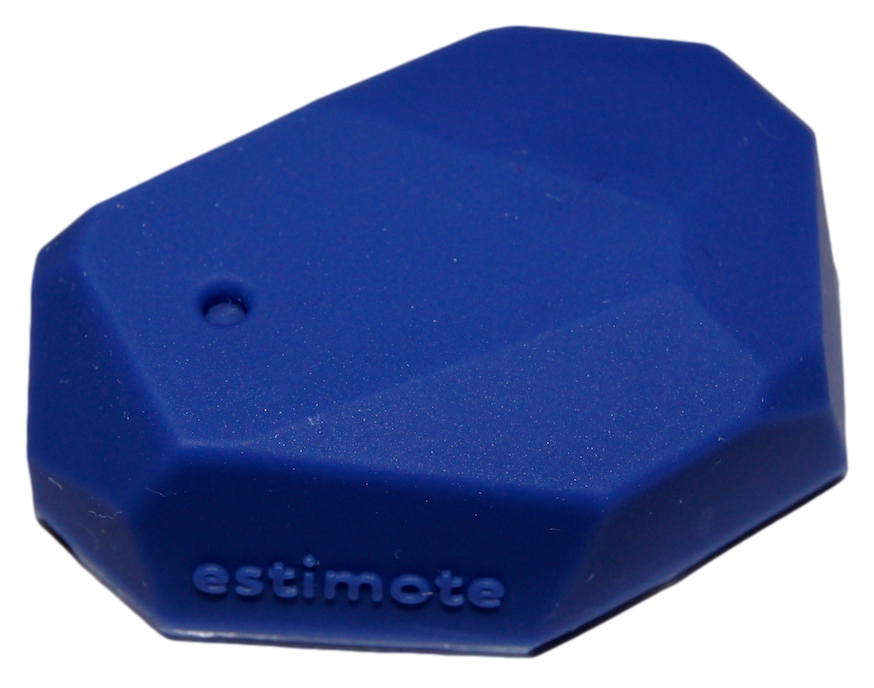
\includegraphics[scale=0.15]{pictures/estimote-beacon-outside}
		\caption{Außenhülle}
		\label{estimote-outside}
	\end{minipage}
	\hspace{2cm}
	\begin{minipage}[t]{5cm}
			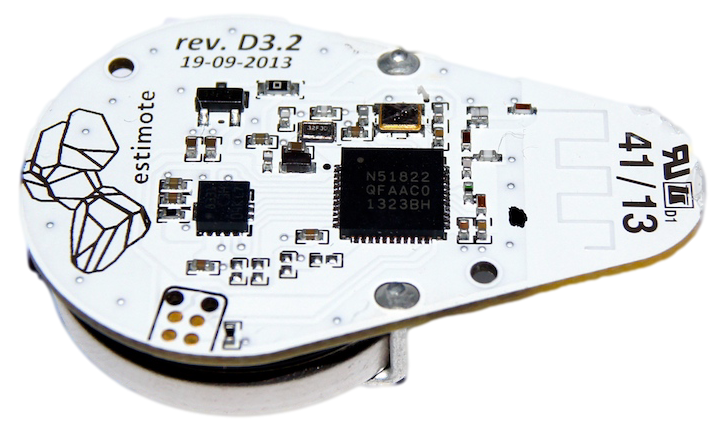
\includegraphics[scale=0.2]{pictures/estimote-beacon-inside}
			\caption{Chipsatz mit Bluetooth-Modul}
			\label{estimote-inside}
		\end{minipage}
		\caption{Ein iBeacon der Firma ''estimote''}{} 
\end{figure}

%%%%%%%%%%%%%%%%%%%%%%%%%%%%%%%%%%%%%%%%%%%%%%%%%%%%%%%%%%%%
\section{iOS und Xcode}
\label{sec:technologies:iosandxcode}
%%%%%%%%%%%%%%%%%%%%%%%%%%%%%%%%%%%%%%%%%%%%%%%%%%%%%%%%%%%%


%%%%%%%%%%%%%%%%%%%%%%%%%%%%%%%%%%%%%%%%%%%%%%%%%%%%%%%%%%%%
\section{CoreLocation-Framework}
\label{sec:technologies:corelocation}
%%%%%%%%%%%%%%%%%%%%%%%%%%%%%%%%%%%%%%%%%%%%%%%%%%%%%%%%%%%%


%%%%%%%%%%%%%%%%%%%%%%%%%%%%%%%%%%%%%%%%%%%%%%%%%%%%%%%%%%%%
\subsection{iBeacons-API}
\label{sec:technologies:iosandxcode:ibeaconsapi}
%%%%%%%%%%%%%%%%%%%%%%%%%%%%%%%%%%%%%%%%%%%%%%%%%%%%%%%%%%%%

%%%%%%%%%%%%%%%%%%%%%%%%%%%%%%%%%%%%%%%%%%%%%%%%%%%%%%%%%%%%
\subsection{Weitere API's}
\label{sec:technologies:iosandxcode:otherapis}
%%%%%%%%%%%%%%%%%%%%%%%%%%%%%%%%%%%%%%%%%%%%%%%%%%%%%%%%%%%%


%%%%%%%%%%%%%%%%%%%%%%%%%%%%%%%%%%%%%%%%%%%%%%%%%%%%%%%%%%%%
\section{CoreData-Framework}
\label{sec:technologies:coredata}
%%%%%%%%%%%%%%%%%%%%%%%%%%%%%%%%%%%%%%%%%%%%%%%%%%%%%%%%%%%%